
% ----- ASY SETUP ----------------------------
\begin{asydef} 
defaultpen(fontsize(10));
settings.outformat="pdf";
usepackage("amsmath");
usepackage("amssymb"); 
usepackage("giambattista");
texpreamble("\renewcommand{\vec}[1]{\mathbf{#1}}");
texpreamble("\let\e\relax");
texpreamble("\DeclareMathOperator{\e}{e}"); 
import x11colors;
pen softblue = rgb(0.92,0.95,0.99);
pen softred = rgb(0.99, 0.92, 0.91);
pen softyellow = rgb(0.98, 0.98, 0.9);
pen softgreen = rgb(0.96, 0.995, 0.98);
settings.render = 8; 
\end{asydef}

\newsavebox{\asybox}
\def\asydir{asy3d}

%---- PRINT AUTHOR INFO ------------------
\makeatletter                       
\def\printauthor{%                  
  {\large \@author}}              
\makeatother
%\author{%
 % {\Large \textit{Samuel S.\ Watson}} \\ \vspace{2mm} {sswatson@brown.edu}
 % }

\author{\Large \textit{Samuel S.\ Watson}}

%----- SIDE ICONS ------------------------
\newcommand{\milink}[3][-7.5mm]{\sidenote{\href{http://mathinsight.org/#2}{\mi} on #3}[#1]}
\newcommand\cocalc[1][-2pt]{\raisebox{#1}{
\includegraphics[width=12pt]{figures/cocalc_new}}}
\newcommand\tbob[1][-2pt]{\raisebox{#1}{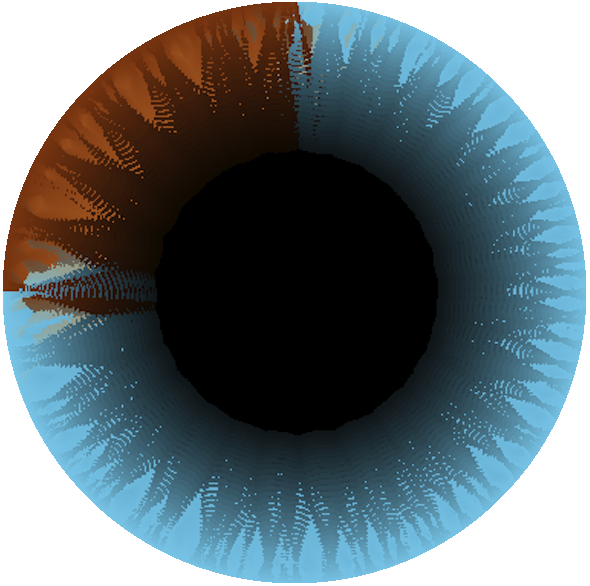
\includegraphics[width=12pt]{figures/3b1b_new}}}
\newcommand\mi[1][-2pt]{\raisebox{#1}{
\includegraphics[width=12pt]{figures/mathinsight}}}


\definecolor{titlepagecolor}{cmyk}{1,.60,0,.40}

\usetikzlibrary{decorations.fractals}

\newcommand\titlepagedecoration{%
  
  \begin{tikzpicture}[remember picture,overlay,shorten >= -10pt]

\coordinate (aux1) at ([xshift=8pt,yshift=-400pt]current page.north east);
\coordinate (aux2) at ([xshift=8pt,yshift=-125pt]current page.north east);
\coordinate (aux3) at ([xshift=50, yshift=-475pt]current page.north east);
\coordinate (aux4) at ([xshift=-10pt,yshift=300pt]current page.south west);
\coordinate (aux5) at ([xshift=-10pt,yshift=455pt]current page.south west);
\coordinate (aux6) at ([xshift=300pt,yshift=-15pt]current page.south
west);
\coordinate (aux7) at ([xshift=0pt,yshift=80pt]current page.south west);

\begin{scope}[decoration=Koch snowflake]

\draw[titlepagecolor!20,line width=2pt]
decorate{decorate{decorate{decorate{(aux3) -- ++(137:7) -- ++(57:7)}}}}; 

\draw[titlepagecolor!30,line width=1.5pt]
decorate{decorate{decorate{decorate{(aux7) -- ++(40:8) -- ++(-5:8)}}}};

\draw[titlepagecolor!80,line width=1pt,fill = softblue]
decorate{decorate{decorate{decorate{(aux6) -- ++(80:10) --
        (aux1)}}}}--
(current page.south east) -- cycle ;

\draw[titlepagecolor!40,line width=1pt]
decorate{decorate{decorate{(aux2) -- ++(115:3) -- ++(70:3)}}};

\draw[titlepagecolor!50,line width=1pt]
decorate{decorate{decorate{decorate{(aux2) -- ++(115:9)}}}};

\draw[titlepagecolor!30,line width=3pt,rounded corners=6pt]
       (aux5) -- ++(45:2) -- ++(135:2); 

\draw[titlepagecolor!60,line width=4pt,rounded corners=6pt]
(aux4) -- ++(45:5) -- ++(135:5);

\end{scope}
\end{tikzpicture}%
}
